\subsection{Movimiento de un objeto unido a un resorte}

  \PN \textit{Posición de equilibrio}: Cuando el resorte no está estirado ni comprimido el bloque queda en reposo.

  \vspace{3mm}
  \PN Consideremos el siguiente modelo:

  \begin{figure}[H]
  \centering
    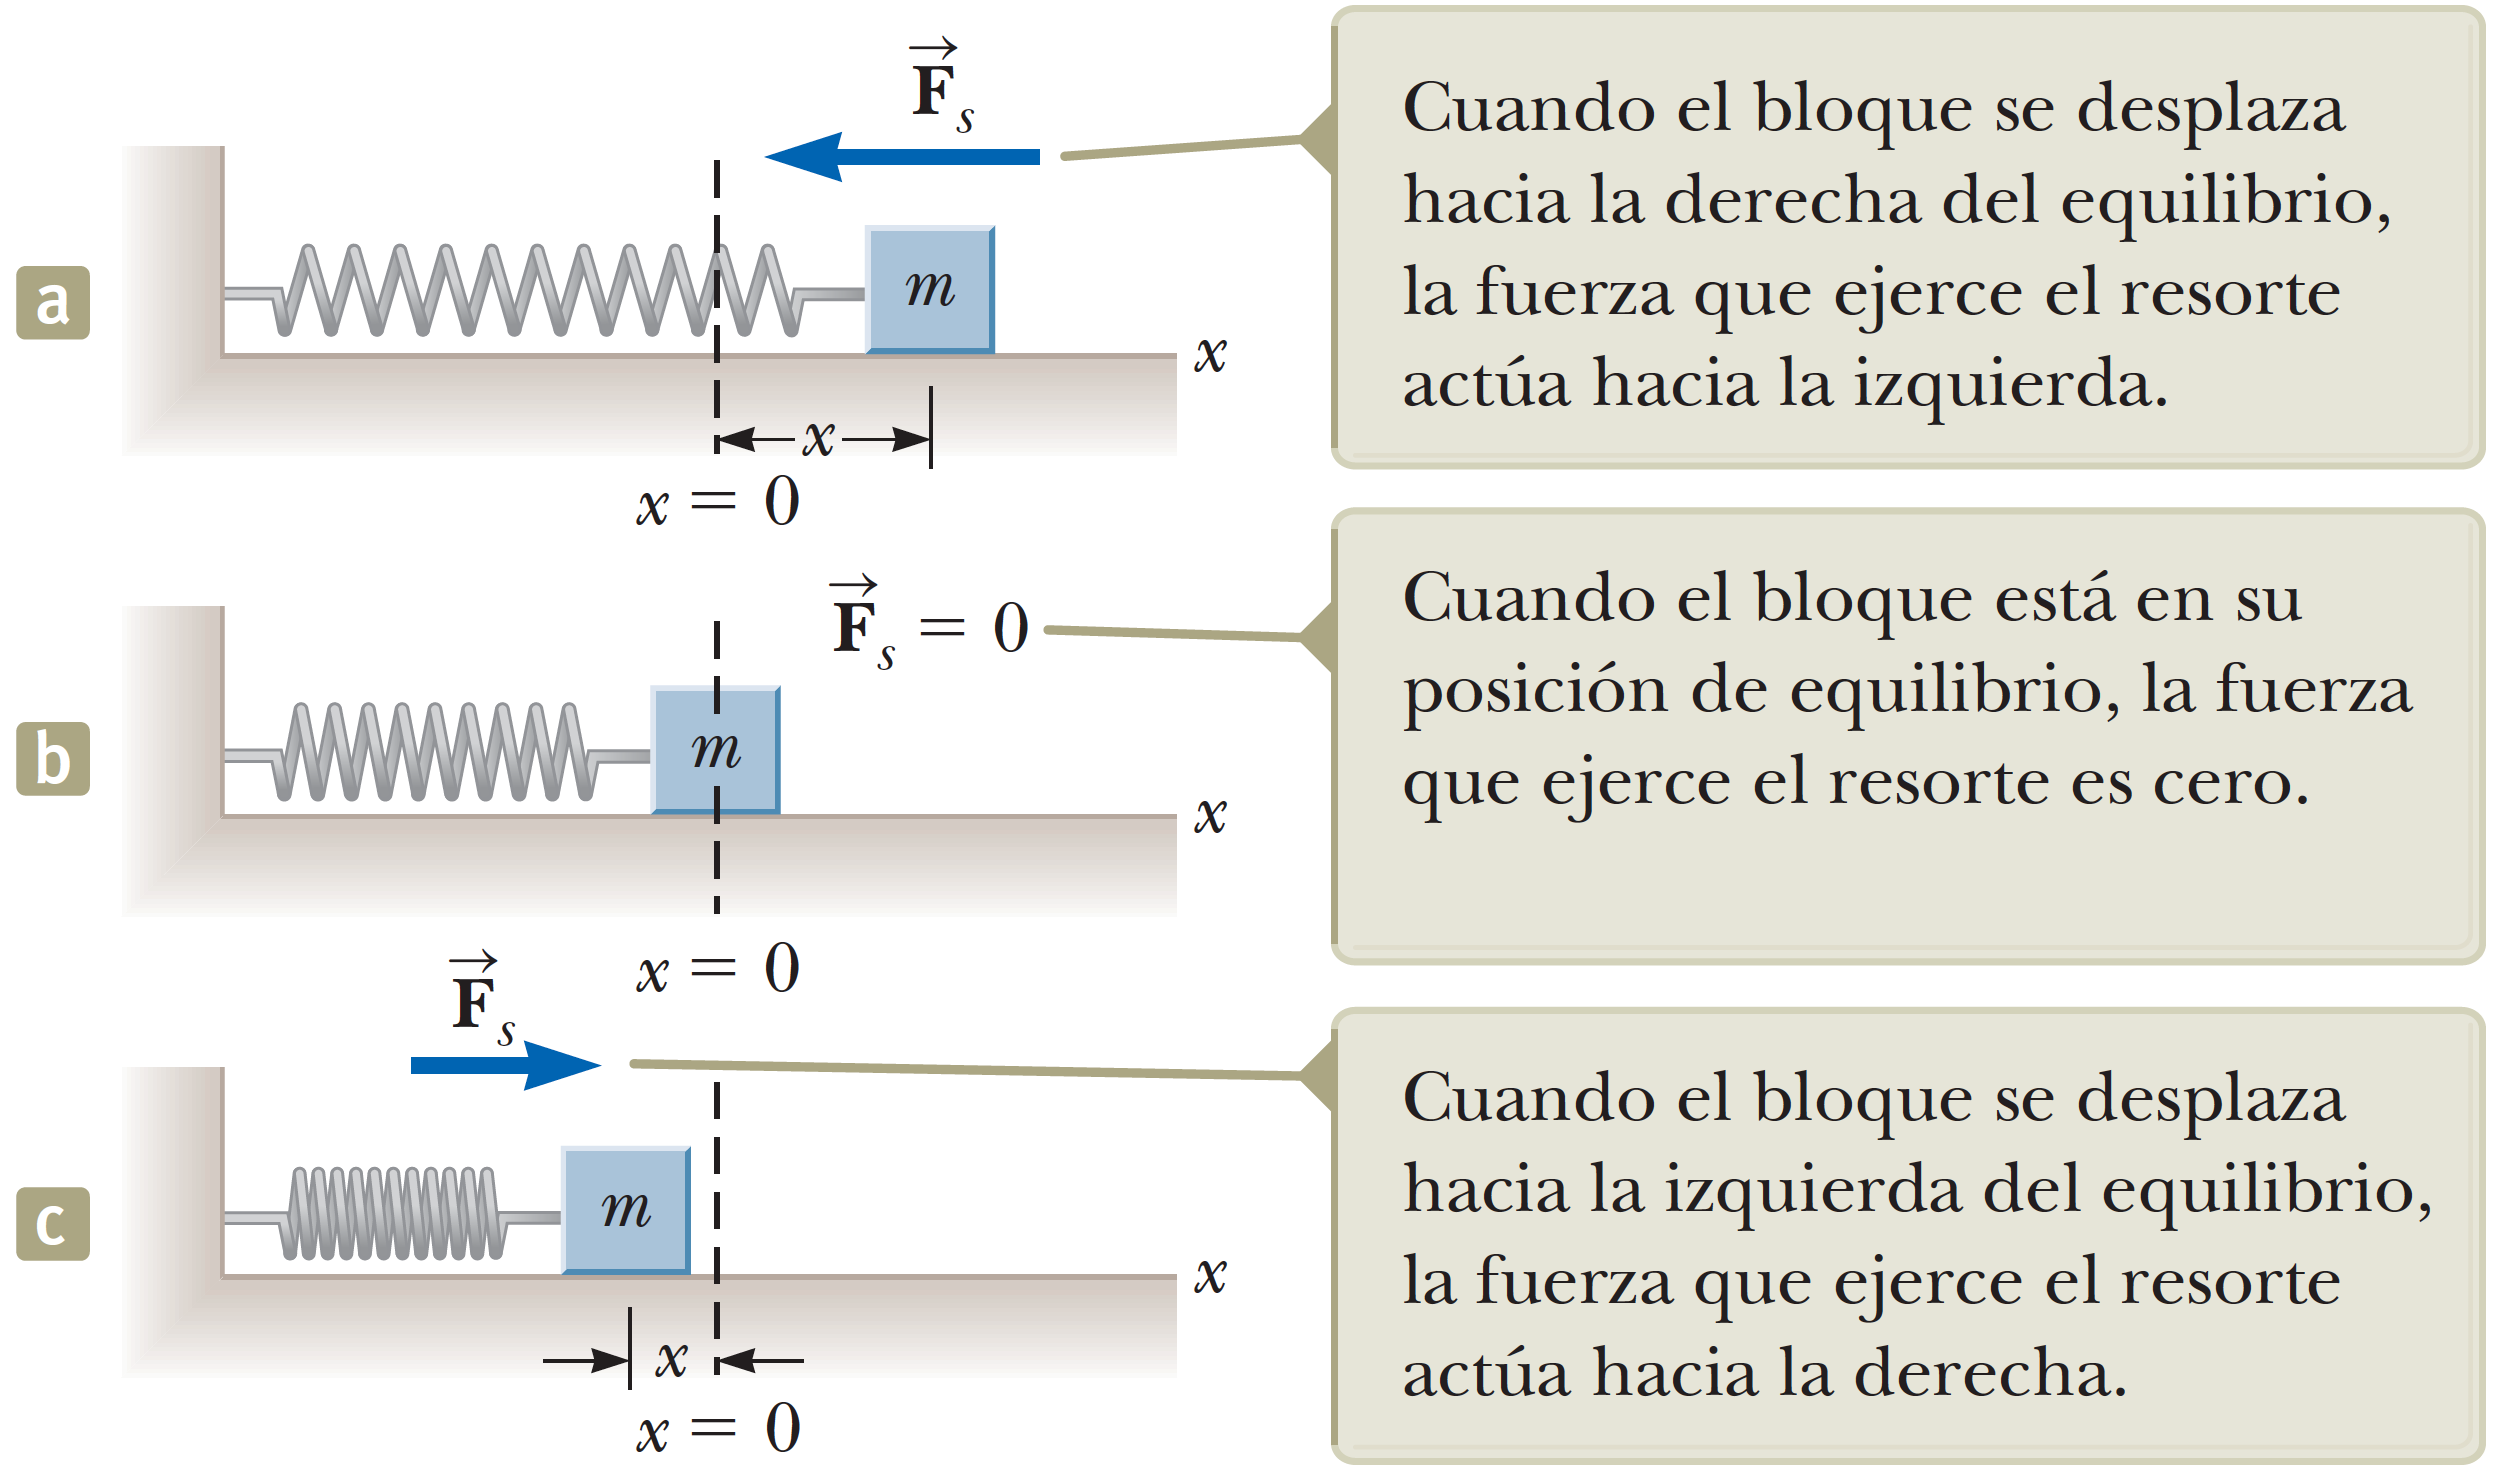
\includegraphics[width=0.6\textwidth]{2/figure_1}
    \caption{Bloque unido a un resorte móvil sobre una superficie sin fricción.}
  \end{figure}

  \PN Cuando el bloque se desplaza a una posición x, el resorte ejerce sobre el bloque una fuerza que es proporcional a
  la posición y está dada por la \textbf{ley de Hooke}:
  \begin{equation}\label{eq:1}
    \underbrace{F_{s}}_{\text{fuerza restauradora}} = -\underbrace{k}_{\text{constante elástica}}\underbrace{x}_{\text{compresión}}
  \end{equation}
  \PN Cuando el bloque es desplazado desde el punto de equilibrio y se suelta, éste es una partícula bajo una fuerza
  neta y, en consecuencia, experimenta una aceleración. Al aplicar la segunda ley de Newton al movimiento del bloque,
  con la ecuación \ref{eq:1} que proporciona la fuerza neta en la dirección x, se obtiene:
  \begin{eqnarray*}
    \Sigma \ F_{x} = ma_{x} &\rightarrow& -kx = ma_{x} \\
    a_{x} &=& \frac{-k}{m}x
  \end{eqnarray*}

  \PN Se dice que los sistemas en los cuales la aceleración del bloque es proporcional a su posición, y la dirección de
  la aceleración es opuesta a la dirección del desplazamiento del bloque desde el equilibrio exhiben \textbf{movimiento
  armónico simple}.

  \PN En ausencia de fricción este movimiento idealizado continuará por siempre porque la fuerza que ejerce el resorte
  es conservativa.
